\chapter{Materials and methods} \label{material_methods}

\section{Research area} \label{research_area}
The Canton of Zug was chosen by the author - who was raised in Cham - as the area of interest since important local knowledge was already present. The specific areas for which social media data (SMD) was acquired are visible in the map below (see figure \ref{fig:research_area}). The turquoise area resembles the political border of the Canton of Zug for which SMD for the social media platforms (SMP) Flickr and Foursquare were collected. The purple area is included in the above mentioned perimeter of the Canton of Zug and consists of three major areas. In the North lies the \lq Lorzenebene\rq (plane of the river Lorze). This area is of special interest to the cantonal authorities due to its local recreation value. An overall concept - named \lq Leitbild Lorzenebene\rq has been created for it which was used as reference in this thesis \cite{BaudirektiondesKantonsZug2012LeitbildBericht}. The second area resembles the jurisdiction of the City of Zug which partly encompasses the \lq Lorzenebene\rq . This area is distinctive by its internal urban gradient which increases towards the city centre as well as the long reaching lake side. The last area furthest South consists of the three mountains \lq Zuger-, Walchwiler-, Rossberg\rq which are likewise part of an development concept \cite{Berchtold2011EntwicklungsleitbildRossberg} of the Canton of Zug due to their sport and recreation value. \\
There is no perimeter concordance due to varying constraints in the data acquisition between the different social media platforms which will be illustrated further down in section \ref{data_acquisition}.

\begin{figure}[h]
   \centering
   \includegraphics[width=0.75\textwidth]{img/overview_research_area_w_Lorzenebene.eps}
   \caption{Overview over the data acquisition perimeters}
   \label{fig:research_area}
\end{figure}


\section{Data acquisition and composition} \label{data_acquisition}
The following subsections will elaborate on the data-acquisition process and the data-composition of the three SMP used in this thesis. 

\subsection{Instagram} \label{instagram}
Instagram is a SMP which supports the sharing of geo-referenced image and video content. The platform is mostly financed by web-advertisement and belongs to \textit{Facebook Inc.} It can be accessed via the URL \texttt{https://www.instagram.com/} or the corresponding mobile application.
Instagram held roughly 2\rq529\rq000 users in Switzerland on January 2019 which accounted for 29.4\% of its population. People aged 25 to 34 were the largest user group (780\rq 000). The gender distribution was at 49.4\% women and 50.6\% men \cite{NapoleonCat2019NoTitle}. This popularity was the determining factor that lead to including Instagram data into this thesis.\\

\subsubsection{Query} \label{netlytic}
Licensed Instagram data of the research area visible in figure \ref{fig:research_area} has been collected via the cloud-based text and social media analyser \textit{Netlytic}. \textit{Netlytic} can be accessed via \texttt{https://netlytic.org/} and allows for hashtag (\# + keyword) or location driven queries. Former allows to search for Instagram media objects by providing decisive keywords which are preceded by a \lq \#\rq. The latter was used in the scope of this thesis which allows location based query for Instagram media objects of public accounts in a 5km radius around a given point. The used \textit{Netlytic} query points with their given perimeter are visible in figure \ref{fig:research_area}. The exact latitude / longitude coordinate pairs are the following:\\
\begin{enumerate}
  \item 47.177068, 8.494803
  \item 47.129913, 8.533604
  \item 47.104457, 8.570291
\end{enumerate}

\subsubsection{Time-span} \label{Instagram_timespan}
Data collection has been continuously performed over all three queries from the 30.09.2018 till the 11.12.2018. Due to the retirement of the Instagram Application Program Interface (API) on the 11.12.2018 \cite{Instagram2018InstagramRetirement} this period could not be extended.

\subsubsection{Data} \label{Instagram_data}
The data-collection accounted for 28\rq246 raw Instagram media objects. After the dominant authors and bulk-upload data-processing steps referenced further down (see chapter (\ref{data_processing}) 11\rq777 remained.
The data provided by \textit{Netlytic} came in the Comma Separated Values (CSV) format. Every media object was provided with the following information entities with the appropriate PostgreSQL data type in square brackets:
\begin{itemize}
    \item id : Unique media object identifier. [varchar(30)] if the media object contains location information, [numeric(20)] if not.
    \item latitude and longitude: coordinate information in the WGS84 reference system [double precision]
    \item link : URL to the actual media object on \texttt{https://www.Instagram.com/} [text]
    \item media-link : URL directing solely to the image content [text]
    \item publication date : Date and time when the media object was uploaded with the data-format YYYY-MM-DD HH:MM:SS [timestamp]
    \item author : The Instagram username of the media object author [text]
    \item title : User generated media object title [text]
    \item description : User generated media object description [text] 
    \item like-count : Amount of likes the media object received on the SMP Instagram
\end{itemize}

Additional location related information (address) was gathered for all the media objects via the official Instagram API. More information can be found in chapter \ref{sec: XXXXX}


\subsection{Flickr} \label{flickr}
Flickr is photo sharing website (\texttt{https://www.flickr.com/}) that allows users to upload geo-reverenced images similar to Instagram. The corresponding free of charge Flickr API gives access to the entire database of Flickr media objects since the launch of the platform in the year 2005. The popularity of Flickr according to the\lq Alexa Global Rank\rq lies at 349 \cite{Alexa.com2019AlexaFlickr} which is significantly lower than to the one of Instagram which lies at 16 \cite{Alexa.com2019AlexaInstagram}. Flickr still plays an important role also as data foundation for scientific studies due to the simple and unbounded data-access. <ADD REFERENCES>
DEMOGRPAHIC INFORMATION
WHY WAS IT CHOSEN
\subsubsection{Query} \label{flickr_query}
The entire Flickr database was queried via the publicly accessible official Flickr API. Media objects with a geo-reference-accuracy level of 12 or higher (maximum of 16) were of interest which resolves to city level up to street level. Queries were conducted by inputting several different bounding boxes which together cover the entire perimeter of the legal boundaries of the canton of Zug. Each bounding box was defined by two coordinate pairs, describing the bottom left and top right corner of a rectangle. This process of subdividing the area was necessary due to a maximum return threshold of 4\rq000 media objects per request. Therefore, to ensure the acquisition of the entire available data-set each bounding box had to hold less than 4\rq000 media objects.
\subsubsection{Time-span} \label{flickr_timespan}
The all the individual bounding-box API requests described above were queried for the time-spawn 2005 (launch of the SMP Flickr) until the 23rd of November 2018. 
\subsubsection{Data} \label{flickr_data}
The data that was returned by the Flickr API was in the JavaScript Object Notation (JSON) format. The following information has been extracted for every Flickr media object:\\

\begin{itemize}
    \item id : Unique media object identifier [bigint]
    \item latitude and longitude: coordinate information in the WGS84 reference system [double precision]
    \item link : URL to the actual media object in the format \texttt{https://www.flickr.com/photos/[author]/[ID]/} [text]
    \item date taken : Time-stamp from the image meta-data stating when it was taken. 
    \item publication date : Time-stamp when the media object was uploaded to Flickr with the data-format MM/DD/YYYY HH:MM:SS [time-stamp]
    \item author : The Flickr username of the media object author [text]
    \item author id : Unique author identifier [text] 
    \item author origin : User given geographical information regarding the authors origin [text]
    \item title : User generated media object title [text]
    \item description : User generated media object description [text]
    \item tags : Keywords similar to Instagram hashtags that describe the media object [text]
    \item views : Amount of media object calls [bigint]
    \item favorites : Amount of approves - similar to \lq likes\rq on Instagram - a media object received by other Flickr users [bigint]
\end{itemize}

Additional location related information (address and location type) was gathered for all the media objects via the Google Geocoding API. More information can be found in chapter \ref{sec: XXXXX}

\subsection{Foursquare} \label{foursquare}
Foursquare is a platform which enables users to rate and share their visits and experiences to certain establishments (referred to as venues). All the stored \lq infrastructure\rq which is categorised into different sectors such as \lq Travel & Transport\rq, \lq Arts and Entertainment\rq but also \lq Outdoors & Recreation\rq can be accessed via the official Foursquare API.
DEMOGRAPHIC INFORMATION
WHY WAS IT CHOSEN
\subsubsection{Query} \label{foursquare_query}
The following two API endpoints which return different information were used for this thesis.
\paragraph{Venue search (regular endpoint)} \label{foursquare_endpoint1}
The first step of the information acquirement involved a spatial search for venue ids of the category \lq Outdoors & Recreation\rq that lie within the research area boundaries. This request was done with the regular venue search API endpoint. There was a limitation to the maximum number of results per request, similar to the bounding box request of Flickr. Therefore, a similar spatial subdivision of the research areas was used to query all the available venues, so that each individual request returned less than 50 results.
\paragraph{Acquiring venue details (premium endpoint)} \label{foursquare_endpoint2}
To obtain more specific information about each venue, a second (premium) Foursquare API endpoint was used. This venue details endpoint only allowed 50 requests per day for regular users which spread the data acquisition over 9 days. Insight among others on a more concrete subcategory description, the formatted address, the user rating as well as if the venue was verified or not was the result.
\subsubsection{Data verification} \label{foursquare_data_verification}
Of all 405 venues located inside the canton of Zug, 13 (3.2\%) are verified according to the data provided by the foursquare API. The remaining non-verified venues of the categories: scenic outlook, playground, athletics & sport, farm, (nudist) beach, lake, trail, golf course, mountain, campground, bathing area, outdoors & recreation, harbour, recreation centre, dog run, forest, pedestrian plaza, waterfront, basketball court, river, bike trail and skate park were evaluated by the author - who grew up in the area - to its best knowledge. XY venues belonged to said categories of which XY were verified by the author of this thesis.
\subsubsection{Data} \label{fq_data}






